\documentclass[conference]{IEEEtran}
\IEEEoverridecommandlockouts
% The preceding line is only needed to identify funding in the first footnote. If that is unneeded, please comment it out.
\usepackage{cite}
\usepackage{amsmath,amssymb,amsfonts}
\usepackage{algorithmic}
\usepackage{graphicx}
\usepackage{textcomp}
\usepackage{xcolor}
\usepackage{bm}
\def\BibTeX{{\rm B\kern-.05em{\sc i\kern-.025em b}\kern-.08em
    T\kern-.1667em\lower.7ex\hbox{E}\kern-.125emX}}
\begin{document}

\title{Crowd Counting Using WiFi\\
%{\footnotesize \textsuperscript{*}Note: Sub-titles are not captured in Xplore and
%should not be used}
}

\author{\IEEEauthorblockN{1\textsuperscript{st} Andreas Rayzik}
\IEEEauthorblockA{\textit{dept. name of organization (of Aff.)} \\
\textit{name of organization (of Aff.)}\\
City, Country \\
email address}

}

\maketitle

\begin{abstract}
By using WiFi as a medium for estimating the number of people in a room or in a certain area, a great potential of cost-saving and simplification of deployment can be leveraged.
\vspace{80mm}
\end{abstract}

\begin{IEEEkeywords}
WiFi, IoT, people counting, crowd counting
\end{IEEEkeywords}

\section{Introduction}
The main motivations behind performing crowd counting in buildings are the applications of energy efficiency, customer guidance in retail stores and traffic optimization "smart" cities. [citation needed] By estimating the number of people in a building, the demand for energy-intensive appliances like air conditioning or heating can be calculated and regulated. By reducing the operation of the appliances for a low number of people, a substantial amount of energy can be saved compared to an unregulated operation. 
\par
In customer guidance applications, people could receive information or advertisement based on their proximity to specific products in a store. With the user's consent, this data could be connected to personal characteristics to increase the relevancy of the provided information. For the retail operator, the motivation is to improve user experience and to increase sales counts. For the customer, the additional information can lead to better informed purchase decisions and a feeling of being guided while navigating a store. [citation needed]
\par
Motivations for using WiFi in particular are the low cost of using off-the-shelf components like consumer WLAN routers and transceiver sticks. Off-the-shelf hardware comes with approval by the Federal Communications Commission, which allocates frequency ranges and checks for maximum signal strengths [citation needed]. If one were to develop one's own wireless technology for the problem, an assignment of the used frequency range and maximum signal strength would first be mandatory to apply the solution in public places. The process of assignment and checking is complex and time-consuming. This is the reason why using off-the-shelf hardware can save a large amount of resources. (TODO: all methods device-free?)
\par
The following work will provide a history of approaches described in research literature. Additionally, a quantitative comparison between the approaches will be shown. Further, the work tries to give an explanation why the problem has not been solved yet despite many years of research. The main contribution of this paper will be a comparison to approaching the crowd counting problem with either WiFi technology, camera sensors or RFID sensors. This comparison will take the factors of accuracy, cost, privacy and perceived privacy by the target person into account. 


\section{Challenges}
The hypothetical best solution would be a system with a deployment as easy as setting up one low-cost device per building, in an arbitrary location inside the building, while requiring no manual calibration and minimal automatic calibration. Research has shown that reaching these goals comes with a complicated trade-off and requires creativity and high engineering ingenuity. 
\par
In any environments that are not free of obstructions like walls, furniture, people or animals, WiFi signals propagate in a manner that is very hard to predict. Areas of constructive inferences and destructive inferences can change the signal strength for a receiver significantly. (TODO: How much? 0 to double?) When setting up a WLAN router for a home or a public building, positioning of the router is important. Slight changes in position can mean large changes in signal coverage for the building. Especially coverage of frequented areas is desirable. As WiFi signals consist of electromagnetic radiation, its interference pattern is shaped by its wavelength. The wavelength $\lambda$ can be calculated by: $$\lambda = \frac{c}{f}$$ With the speed of light $c$, the wavelength evaluates to approximately 12.5cm for 2,4GHz WiFi and approximately 6.25cm for 5GHz WiFi respectively.

\par
Table \ref{table_overview} provides an overview of the features of the described techniques for crowd counting that have been developed, sorted chronologically.
\begin{table*}
\caption{Overview of techniques}
\label{table_overview}
\centering
\begin{tabular}{c || c || c || c || c}
\hline
\bfseries \textbf{Author} & \textbf{Publication} & \bfseries\textbf{\# Nodes} & \bfseries \textbf{Max. \# People} & \bfseries \textbf{Calibration} \\
\hline
Yuan et al. & 2011 & 16 & Low/Medium/High & Not mentioned \\
\hline
Xu et al. & 2013 & 22 & 4 (+ location) & Little (Empty room RSS meas.) \\
\hline
Xi et al. & 2014 & 38 & 30 & Extensive \\
\hline
Yoshida/Taniguchi & 2015 & 11 & 7 & Extensive \\
\hline
Depatla et al. & 2015 & 2 & 10 & Little \\
\hline
Domenico et al. & 2016 & 2 & 7 & Extensive \\
\hline
Depatla/Mostofi & 2018 & 2 & 20 & Very little
\end{tabular}
\end{table*}
The feature "calibration" is meant to encompass methods like measuring the signal strength for specific densities of people beforehand, 
As can be seen in \ref{table_overview}, a rough trend has been to reduce the number of nodes needed as well as the calibration necessary.
\par
Bla
\subsection{Crowd Density Estimation Using Wireless Sensor Networks}
Yuan et al. \cite{Yuan} use Wireless Sensor Networks (WSN) to achieve an estimate of the crowd density in a room. A calibration step and a detection step are being iterated in pairs. They validate their approach by deploying a network of 16 wireless sensors. 
\par
The network uses the Collection Tree Protocol (CTP) \cite{ctp}. The CTP is required to collect the data gathered by the sensors reliably and efficiently. Moreover, it aims to minimize energy consumption to extend the sensors' battery lives. It extends the distance vector routing protocol by three additional mechanisms in order to adapt to the special conditions in highly dynamic wireless networks.
\begin{itemize}
\item Information from the physical layer, network layer and link layer are combined to estimate the link quality between two nodes with a resolution of four bits.
\item To detect datapaths that have become unreliable, data packets contain the transmitter's local cost estimate. The expected transmissions (ETX) can be used as a cost metric. When a packet is being forwarded, the transmitter's cost is expected to always be greater than the forwarding node's own cost. A deviation from this assumption hints at a loop in the network.
\item Adaptive Beaconing deals with the compromise of choosing a large or small interval for sending control packets. A large interval saves bandwidth and energy, but makes the network slower to react to adverse wireless dynamics. Adaptive beaconing changes the interval according to the consistency and problem rate in the network.
\end{itemize}
In the detection step, the K-means algorithm is used to cluster the data from the WSN into density levels of low, medium of high. The thresholds for these levels are set arbitrarily and can be changed. For the number of clusters K, the best convergence was achieved with $K=2$.


\subsection{SCPL: Indoor Device-Free Multi-Subject Counting and Localization Using Radio Signal Strength}
Xu et al. \cite{Xu} use the long-range property of radio signals to deploy a counting technique in two large indoor settings with 150$m^2$ and 400$m^2$. They can detect up to four subjects which is a low number compared to the other works, but it includes the subject's location. The abbreviation SCPL refers to the way of counting the number of subjects sequentially while doing the localization in parallel. They model the human trajectories as a state transition process and use Conditional Random Fields (CRF) to attack the localization problem.
\par
As a calibration, the RSS values for every link are measured when the rooms are empty. This data can then be used to determine how much a subject's presence alters the RSS value in a cell. For the presence of multiple subjects, a hypothesis is being made that it will "affect a larger number of spatially distributed radio links, [...] also lead to a higher level of RSS change on these links." Instead of using the RSS mean difference as a metric, the authors propose the absolute RSS mean difference. As the reason for this, they state that the additional presence of another subject might not always weaken a link. Due to multipath effects, it might actually strengthen a link. Thus, the RSS mean difference is not always positive. The absolute RSS mean difference represents the total energy change more suitably.
\par
The researchers exploit the fact that human movement constitutes a continuous trajectory. They model the movement as a CRF, which is a type of discriminative undirected probabilistic graphical model \cite{crf}. CRFs are comparable to hidden Markov models (HMMs), but possess for example the advantage to be able to relax strong independence assumptions. CRFs models the probability $$p(\bm{Y}|\bm{X})$$ for the jointly distributed random variables $\bm{Y}$ and $\bm{X}$. The aim is to maximize the likelihood that a subject is located in the same cell $i$ that was estimated. The cells correspond to the states there were defined as $\bm{Y}$.

\subsection{X-Ray Vision with Only WiFi Power Measurements Using Rytov Wave Models}
Depatla, Buckland and Mostofi published a paper in 2015 \cite{DepatlaMostofi2015} where they introduce modelling of wave propagation to enable high-resolution see-through imaging. They apply their technique to unmanned, autonomously moving robots and discuss how they improved on the robot positioning and antenna alignment. As this is out of the scope of the current paper, it shall not be explained in further detail. For the wave propagation modelling, Rytov approximations are considered suitable. They are a linearising approximation to Maxwell's equations. Scattering effects are included. They explain that the Wentzel Kramer Brillouin (WKB) approximation often used in X-ray is not suitable for their purposes. It makes an assumption that only holds at high frequencies. The 2,4GHz microwave frequency is low compared to X-ray frequencies. In particular, they state that "Throughout[sic] this paper, high frequency refers to the frequencies at which the size of inhomogeneity of objects is much larger than the wavelength." They go on to lay out the Rytov approximation. It is followed by an explanation of an intensity-only variant of the Rytov Approximation. This is narrowed down further to an intensity-only LOS approximation, that results in the final equation $$P_{LOS} = A\Gamma$$
$P$ is the received power in dBm at $r$. $A$ is a two-dimensional matrix with entries 1 and 0 for cells that are along the LOS for a measurement $i$ or not along the line, respectively. $\Gamma$ is a vector of complex numbers $\alpha$, where $\alpha$ denotes the slowness of the medium that is penetrated by the radio wave at a position vector $r$.
\par
Because there is a much larger number of unknowns in the linearised equations than the number of wireless measurements can provide for, the system is substantially underdetermined. To alleviate this problem, sparse signal processing is introduced. The fact that the spatial variation of objects to be imaged is sparse is exploited. The authors utilize the MATLAB-based solver TVAL3 (TV Minimization by Augmented Lagrangian and Alternating Direction Algorithm). TV stands for Total Variation. It is a mathematical concept that describes roughly an infinitesimal version of the absolute value.
Figure ~\ref{figRytovLOS} is taken from the paper and shows both the experimental setup in the top-left, as well as the performance of the Rytov approximation over simple LOS approximation.
\begin{figure}[htbp]
\centerline{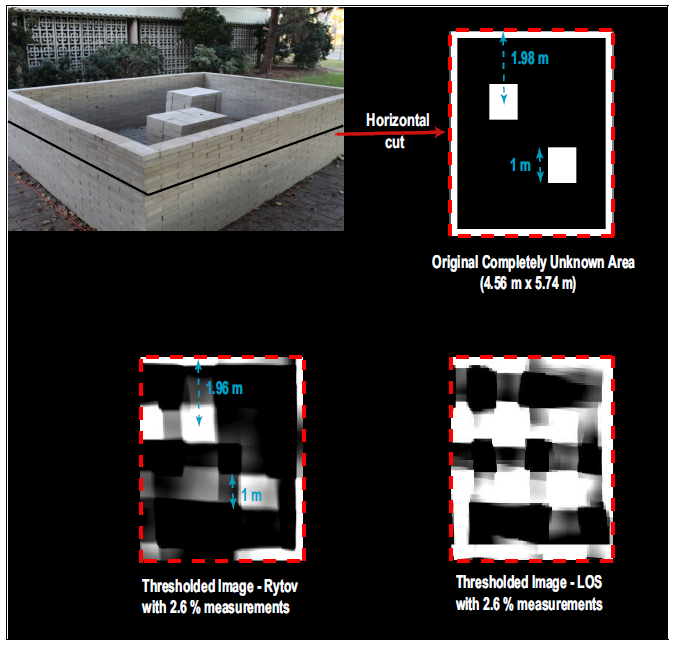
\includegraphics[scale=0.4]{figRytovVsLOS.PNG}}
\caption{Comparison of the Rytov approximation over LOS approximation in the experimental setup \cite{DepatlaMostofi2015}}
\label{figRytovLOS}
\end{figure}
The images visualise very clearly how the Rytov approximations improve the measurement over LOS, which would be hard to describe in words otherwise.
\par
The focus in the paper lies on capturing high-resolution images through walls, using WiFi. To adapt this approach to crowd counting, the sampling rate of the measurements would need to be increased to be able to capture moving persons. Currently, the approach is computationally intensive and takes 3.6 seconds for the Rytov approach on a 3.7GHz CPU. This corresponds to a sampling rate of 0.28Hz. A post-processing step would also have to be added to distinguish people from material obstacles. Thirdly, the number of people to be counted relative to the room size would need to be small enough, since the Rytov approximation exploits the sparsity of spatial variation.

\subsection{Crowd Counting through Walls}
In 2018, Depatla and Mostofi \cite{DepatlaMostofi2018} refined their previous approach to be able to increase the maximum number of people to be counted from 10 to 20. At the same time, the calibration needed was reduced further. They extend their concept to be applicable through walls instead of inside walls. However, their new technique comes with a number of assumptions that make it difficult to be translated to a real-world scenario. A general concept of their approach is depicted in \ref{concept}. The transceiver Tx and the receiver Rx are placed on opposite sides outside the walls of the target room. The direct path between them forms the line of sight (LOS). Up to 20 persons move inside the room. A person's movement is described by the movement speed in x and y coordinates and the angle of direction $\theta$. When one or multiple persons cross the line of sight, the signal is being blocked and attenuated. Also, the presence of persons in the room inevitably leads to multipath effects.
\begin{figure}
\label{concept}
\end{figure}
The researchers define the LOS crossing as an event $E$ and the inter-event times as $T_n$. They then define the discretised motion of a person as a Renewal-type process. Renewal theory is a generalization of Poisson processes, where the holding times can be arbitrary. In our case, the inter-event times $T_n$ represent the holding times. The theory of Poisson processes can be traced back to Markov processes. The inter-event times are identically distributed, but not independent. The authors prove that the probability mass function (PMF) of the inter-event times is an implicit function of the number of people $N$.
\par
They go on to experimentally validate their approach by a setup using a D-link WBR-1310 router as WiFi transceiver, a TP-Link USB card as WiFi receiver and a Raspberry Pi board for controlling the measurements and storing the obtained RSSI values. All of the devices are cheap, off-the-shelf products. Since the measurement run with a sampling rate of 20Hz over the course of 300 seconds, the Raspberry Pi needs to store 6000 values. The experiment is conducted for different numbers of people $$N = (1, 3, 5, 7, 9)$$ up to $N=20$. Further, different kinds of rooms are being tested with varying dimensions and wall materials. Test subjects were also instructed to follow different walking speeds. The authors conclude that their approach achieves and accuracy of less than 1 person difference 81\% of the time and less than a 2 person difference 100\% of the time.
\par
Compared to their previous work from 2015, the new technique is very different. It uses no modelling of wave propagation and thus achieves a much higher sample rate. It uses stationary WiFi transceivers instead of transceivers mounted on autonomous robots. It deals directly with the task of counting people instead of capturing images with radio waves. Both works have in common the fact that they send radio waves through walls.
\section{Discussion}
All of the works presented are limited by the number of people that can be counted at maximum, by the size of the room or other conditions. This makes it difficult to apply them to real-world scenarios. The work by Depatla and Mostofi \cite{DepatlaMostofi} makes particularly strong assumptions. These assumptions and to what degree they prevent the transition to a real-world scenario will be discussed in the following.
\begin{itemize}
\item Random movement patterns by the subjects are assumed. This might be applicable to a situation in which a subject is searching for a certain object, with few clues to where said object might be located. It could also hold in a place like a cafeteria, where people are moving around to greet several acquaintances and search for a free seat. The same goes for a hallway, which connects many places that represent potential starting points or end points for movement. It is problematic in a case in which people partially or in their entirety move as a group with a common goal. Since the authors use a uniform distribution for their motion model, the problem could potentially be tackled by switching to a non-uniform distribution which is adapted to the room and common goals in the room and its context.
\item Subjects are assumed to move independently from each other. This is closely related to the first assumption. It ignores the possibility that a person's movement might influence the movement of others and lead to group dynamics or swarm-like behaviours. This is especially meaningful in a setting where there is a hierarchy among the subjects with one or multiple leaders guiding a group.
\item The previous points lead to the problem of the line of sight (LOS) not actually being crossed. The event of LOS crossing is essential to the authors' technique of estimating the number of people. However, when instead of random, independent movement there is a fixed goal or social group dynamic, the LOS might not be crossed at all. This weakness could be mitigated by adding more pairs of transmitters and receivers which each introduce another LOS per pair.
\item The measurement is required to take at least 300 seconds. During this time, continuous random and independent movement is assumed and no subjects may leave or enter the room. Scenarios with a changing amount of people during the measurement are explicitly stated by the authors as a goal for future work.
\item Another limitation is the number 20 as the maximum of people to be counted. This number is higher than most of the other values in table \ref{table_overview}. Still, when considering a real-world scenario, it is a significant limit and stands in contrast to the advantages of requiring only two wireless nodes and very little calibration. The authors have not provided experimental results for more than 20 people. It is reasonable to expect their technique to work for a higher number when a lower accuracy is acceptable. 
\end{itemize}
Despite all of the problems mentioned, the work makes arguments to how an application in a real-world setting might function. The researchers show that their counting accuracy is robust to different walking speeds. Speeds ranging from casual walking to running have been tested. Moreover, diverse types of rooms have been tested with different dimensions and different wall materials like concrete, plaster or wood.
\par
In general, to facilitate crowd counting for moving subjects, are reasonably high sampling rate is required. Else, the movement of people during one measurement sample could introduce too much noise and make it inaccurate. Subjects that enter and leave an area quickly might not be counted at all. This makes approaches using radio wave modelling difficult to implement. In a three-dimensional setting, models for radio waves are computationally intensive. When high resolution is required, the computational costs are further enlarged. To make such a technique feasible, a highly optimised and parallelised algorithm running on a GPU or FPGA is probably needed. GPUs are processors that offer a much higher degree of potential parallelism compared to a CPU. The disadvantage is that designing a parallelisable algorithm is challenging and programming it for a GPU is difficult as well. FPGAs are chips in which the circuitry itself is programmable for the user. The offer a higher degree of flexibility in contrast to GPUs, but therefore inevitably also increase the complexity of software design.

\section{Conclusion}
Complex wave propagation and decoherence make crowd counting using WiFi a challenging task that is yet to be solved without significant limitations. Techniques refer to a diverse set of basic methods like the Collection Tree Protocol, Conditional Random Fields or Renewal theory. Assumptions made in research literature often do not translate to real-world scenarios.

\section{Prepare Your Paper Before Styling}
Before you begin to format your paper, first write and save the content as a 
separate text file. Complete all content and organizational editing before 
formatting. Please note sections \ref{AA}--\ref{SCM} below for more information on 
proofreading, spelling and grammar.

Keep your text and graphic files separate until after the text has been 
formatted and styled. Do not number text heads---{\LaTeX} will do that 
for you.

\subsection{Abbreviations and Acronyms}\label{AA}
Define abbreviations and acronyms the first time they are used in the text, 
even after they have been defined in the abstract. Abbreviations such as 
IEEE, SI, MKS, CGS, ac, dc, and rms do not have to be defined. Do not use 
abbreviations in the title or heads unless they are unavoidable.

\subsection{Units}
\begin{itemize}
\item Use either SI (MKS) or CGS as primary units. (SI units are encouraged.) English units may be used as secondary units (in parentheses). An exception would be the use of English units as identifiers in trade, such as ``3.5-inch disk drive''.
\item Avoid combining SI and CGS units, such as current in amperes and magnetic field in oersteds. This often leads to confusion because equations do not balance dimensionally. If you must use mixed units, clearly state the units for each quantity that you use in an equation.
\item Do not mix complete spellings and abbreviations of units: ``Wb/m\textsuperscript{2}'' or ``webers per square meter'', not ``webers/m\textsuperscript{2}''. Spell out units when they appear in text: ``. . . a few henries'', not ``. . . a few H''.
\item Use a zero before decimal points: ``0.25'', not ``.25''. Use ``cm\textsuperscript{3}'', not ``cc''.)
\end{itemize}

\subsection{Equations}
Number equations consecutively. To make your 
equations more compact, you may use the solidus (~/~), the exp function, or 
appropriate exponents. Italicize Roman symbols for quantities and variables, 
but not Greek symbols. Use a long dash rather than a hyphen for a minus 
sign. Punctuate equations with commas or periods when they are part of a 
sentence, as in:
\begin{equation}
a+b=\gamma\label{eq}
\end{equation}

Be sure that the 
symbols in your equation have been defined before or immediately following 
the equation. Use ``\eqref{eq}'', not ``Eq.~\eqref{eq}'' or ``equation \eqref{eq}'', except at 
the beginning of a sentence: ``Equation \eqref{eq} is . . .''

\subsection{\LaTeX-Specific Advice}

Please use ``soft'' (e.g., \verb|\eqref{Eq}|) cross references instead
of ``hard'' references (e.g., \verb|(1)|). That will make it possible
to combine sections, add equations, or change the order of figures or
citations without having to go through the file line by line.

Please don't use the \verb|{eqnarray}| equation environment. Use
\verb|{align}| or \verb|{IEEEeqnarray}| instead. The \verb|{eqnarray}|
environment leaves unsightly spaces around relation symbols.

Please note that the \verb|{subequations}| environment in {\LaTeX}
will increment the main equation counter even when there are no
equation numbers displayed. If you forget that, you might write an
article in which the equation numbers skip from (17) to (20), causing
the copy editors to wonder if you've discovered a new method of
counting.

{\BibTeX} does not work by magic. It doesn't get the bibliographic
data from thin air but from .bib files. If you use {\BibTeX} to produce a
bibliography you must send the .bib files. 

{\LaTeX} can't read your mind. If you assign the same label to a
subsubsection and a table, you might find that Table I has been cross
referenced as Table IV-B3. 

{\LaTeX} does not have precognitive abilities. If you put a
\verb|\label| command before the command that updates the counter it's
supposed to be using, the label will pick up the last counter to be
cross referenced instead. In particular, a \verb|\label| command
should not go before the caption of a figure or a table.

Do not use \verb|\nonumber| inside the \verb|{array}| environment. It
will not stop equation numbers inside \verb|{array}| (there won't be
any anyway) and it might stop a wanted equation number in the
surrounding equation.

\subsection{Some Common Mistakes}\label{SCM}
\begin{itemize}
\item The word ``data'' is plural, not singular.
\item The subscript for the permeability of vacuum $\mu_{0}$, and other common scientific constants, is zero with subscript formatting, not a lowercase letter ``o''.
\item In American English, commas, semicolons, periods, question and exclamation marks are located within quotation marks only when a complete thought or name is cited, such as a title or full quotation. When quotation marks are used, instead of a bold or italic typeface, to highlight a word or phrase, punctuation should appear outside of the quotation marks. A parenthetical phrase or statement at the end of a sentence is punctuated outside of the closing parenthesis (like this). (A parenthetical sentence is punctuated within the parentheses.)
\item A graph within a graph is an ``inset'', not an ``insert''. The word alternatively is preferred to the word ``alternately'' (unless you really mean something that alternates).
\item Do not use the word ``essentially'' to mean ``approximately'' or ``effectively''.
\item In your paper title, if the words ``that uses'' can accurately replace the word ``using'', capitalize the ``u''; if not, keep using lower-cased.
\item Be aware of the different meanings of the homophones ``affect'' and ``effect'', ``complement'' and ``compliment'', ``discreet'' and ``discrete'', ``principal'' and ``principle''.
\item Do not confuse ``imply'' and ``infer''.
\item The prefix ``non'' is not a word; it should be joined to the word it modifies, usually without a hyphen.
\item There is no period after the ``et'' in the Latin abbreviation ``et al.''.
\item The abbreviation ``i.e.'' means ``that is'', and the abbreviation ``e.g.'' means ``for example''.
\end{itemize}
An excellent style manual for science writers is \cite{b7}.

\subsection{Authors and Affiliations}
\textbf{The class file is designed for, but not limited to, six authors.} A 
minimum of one author is required for all conference articles. Author names 
should be listed starting from left to right and then moving down to the 
next line. This is the author sequence that will be used in future citations 
and by indexing services. Names should not be listed in columns nor group by 
affiliation. Please keep your affiliations as succinct as possible (for 
example, do not differentiate among departments of the same organization).

\subsection{Identify the Headings}
Headings, or heads, are organizational devices that guide the reader through 
your paper. There are two types: component heads and text heads.

Component heads identify the different components of your paper and are not 
topically subordinate to each other. Examples include Acknowledgments and 
References and, for these, the correct style to use is ``Heading 5''. Use 
``figure caption'' for your Figure captions, and ``table head'' for your 
table title. Run-in heads, such as ``Abstract'', will require you to apply a 
style (in this case, italic) in addition to the style provided by the drop 
down menu to differentiate the head from the text.

Text heads organize the topics on a relational, hierarchical basis. For 
example, the paper title is the primary text head because all subsequent 
material relates and elaborates on this one topic. If there are two or more 
sub-topics, the next level head (uppercase Roman numerals) should be used 
and, conversely, if there are not at least two sub-topics, then no subheads 
should be introduced.

\subsection{Figures and Tables}
\paragraph{Positioning Figures and Tables} Place figures and tables at the top and 
bottom of columns. Avoid placing them in the middle of columns. Large 
figures and tables may span across both columns. Figure captions should be 
below the figures; table heads should appear above the tables. Insert 
figures and tables after they are cited in the text. Use the abbreviation 
``Fig.~\ref{fig}'', even at the beginning of a sentence.

\begin{table}[htbp]
\caption{Table Type Styles}
\begin{center}
\begin{tabular}{|c|c|c|c|}
\hline
\textbf{Table}&\multicolumn{3}{|c|}{\textbf{Table Column Head}} \\
\cline{2-4} 
\textbf{Head} & \textbf{\textit{Table column subhead}}& \textbf{\textit{Subhead}}& \textbf{\textit{Subhead}} \\
\hline
copy& More table copy$^{\mathrm{a}}$& &  \\
\hline
\multicolumn{4}{l}{$^{\mathrm{a}}$Sample of a Table footnote.}
\end{tabular}
\label{tab1}
\end{center}
\end{table}

\begin{figure}[htbp]
\centerline{\includegraphics[scale=0.2]{fig1.png}}
\caption{Example of a figure caption.}
\label{fig}
\end{figure}

Figure Labels: Use 8 point Times New Roman for Figure labels. Use words 
rather than symbols or abbreviations when writing Figure axis labels to 
avoid confusing the reader. As an example, write the quantity 
``Magnetization'', or ``Magnetization, M'', not just ``M''. If including 
units in the label, present them within parentheses. Do not label axes only 
with units. In the example, write ``Magnetization (A/m)'' or ``Magnetization 
\{A[m(1)]\}'', not just ``A/m''. Do not label axes with a ratio of 
quantities and units. For example, write ``Temperature (K)'', not 
``Temperature/K''.

\section*{Acknowledgment}

The preferred spelling of the word ``acknowledgment'' in America is without 
an ``e'' after the ``g''. Avoid the stilted expression ``one of us (R. B. 
G.) thanks $\ldots$''. Instead, try ``R. B. G. thanks$\ldots$''. Put sponsor 
acknowledgments in the unnumbered footnote on the first page.

\section*{References}

Please number citations consecutively within brackets. The 
sentence punctuation follows the bracket \cite{b2}. Refer simply to the reference 
number, as in \cite{b3}---do not use ``Ref. \cite{b3}'' or ``reference \cite{b3}'' except at 
the beginning of a sentence: ``Reference \cite{b3} was the first $\ldots$''

Number footnotes separately in superscripts. Place the actual footnote at 
the bottom of the column in which it was cited. Do not put footnotes in the 
abstract or reference list. Use letters for table footnotes.

Unless there are six authors or more give all authors' names; do not use 
``et al.''. Papers that have not been published, even if they have been 
submitted for publication, should be cited as ``unpublished'' \cite{b4}. Papers 
that have been accepted for publication should be cited as ``in press'' \cite{b5}. 
Capitalize only the first word in a paper title, except for proper nouns and 
element symbols.

For papers published in translation journals, please give the English 
citation first, followed by the original foreign-language citation \cite{b6}.
%TODO more references
\begin{thebibliography}{00}
\bibitem{DepatlaMostofi2018} S. Depatla and Y. Mostofi, ``Crowd Counting Through Walls Using Wifi,'' Phil. Trans. Roy. Soc. London, vol. A247, pp. 529--551, April 1955.
\bibitem{Yuan} Yuan et. al., ``Crowd Density Estimation Using Wireless Sensor Networks'' in Magnetism, vol. III, G. T. Rado and H. Suhl, Eds. New York: Academic, 1963, pp. 271--350.
\bibitem{ctp} O. Gnawali et al., ``Collection Tree Protocol''
\bibitem{crf} J. Lafferty et al., Condit
ional Random Fields: Probabilistic Models for Segmenting and Labeling Sequence Data
\bibitem{DepatlaMostofi2015} Y. Yorozu, M. Hirano, K. Oka, and Y. Tagawa, ``X-Ray Vision with Only WiFi Power Measurements Using Rytov Wave Models'' IEEE Transl. J. Magn. Japan, vol. 2, pp. 740--741, August 1987 [Digests 9th Annual Conf. Magnetics Japan, p. 301, 1982].
\bibitem{b7} M. Young, The Technical Writer's Handbook. Mill Valley, CA: University Science, 1989.
\end{thebibliography}
\vspace{12pt}
\color{red}
IEEE conference templates contain guidance text for composing and formatting conference papers. Please ensure that all template text is removed from your conference paper prior to submission to the conference. Failure to remove the template text from your paper may result in your paper not being published.

\end{document}
